\section{Problematika zobrazovania GPS trás}

\indent \indent Zobrazovanie \acrshort{gps} trás je zásadné pre množstvo aplikácií, od navigácie a mapovania až po analýzu údajov o pohybe. \acrshort{gps} zariadenia získavajú informácie z družíc a používajú trianguláciu na určenie polohy. Tieto informácie sa zhromažďujú vo forme súradníc spolu s časovými údajmi\cite{Hegarty2017}.

Trasu získame spojením súradníc získaných z \acrshort{gps} zariadenia. Problém nastáva, keď sú \acrshort{gps} signály ovplyvnené faktormi ako sú terén, počasie alebo rôznymi prekážkami. Ovplyvnené signály môžu viesť k nepresným alebo chybným údajom\cite{Hegarty2017}. Spojením chybných údajov získame nepresnú trasu, ktorá leží mimo skutočnej, po ktorej sme sa reálne pohybovali.

Keď sa rovnakou trasou prechádza opakovane, údaje z GPS zariadenia môžu vykazovať variabilitu. Pri vizualizácii trás, ktoré sú zaznamenané prejdením rovnakej trasy, môže dôjsť k prekrývaniu a neprehľadnosti v dôsledku odchýlok a nepresností. Prekrývajúce sa trasy je možné vidieť na obrázku \ref{fig:neprehladne-trasy}. Z dôvodu nepresnosti je zložité rozpoznať detaily mapy, ako aj cestnú sieť, čo sťažuje identifikáciu jednotlivých trás.

\begin{figure}[H]
  \centering
  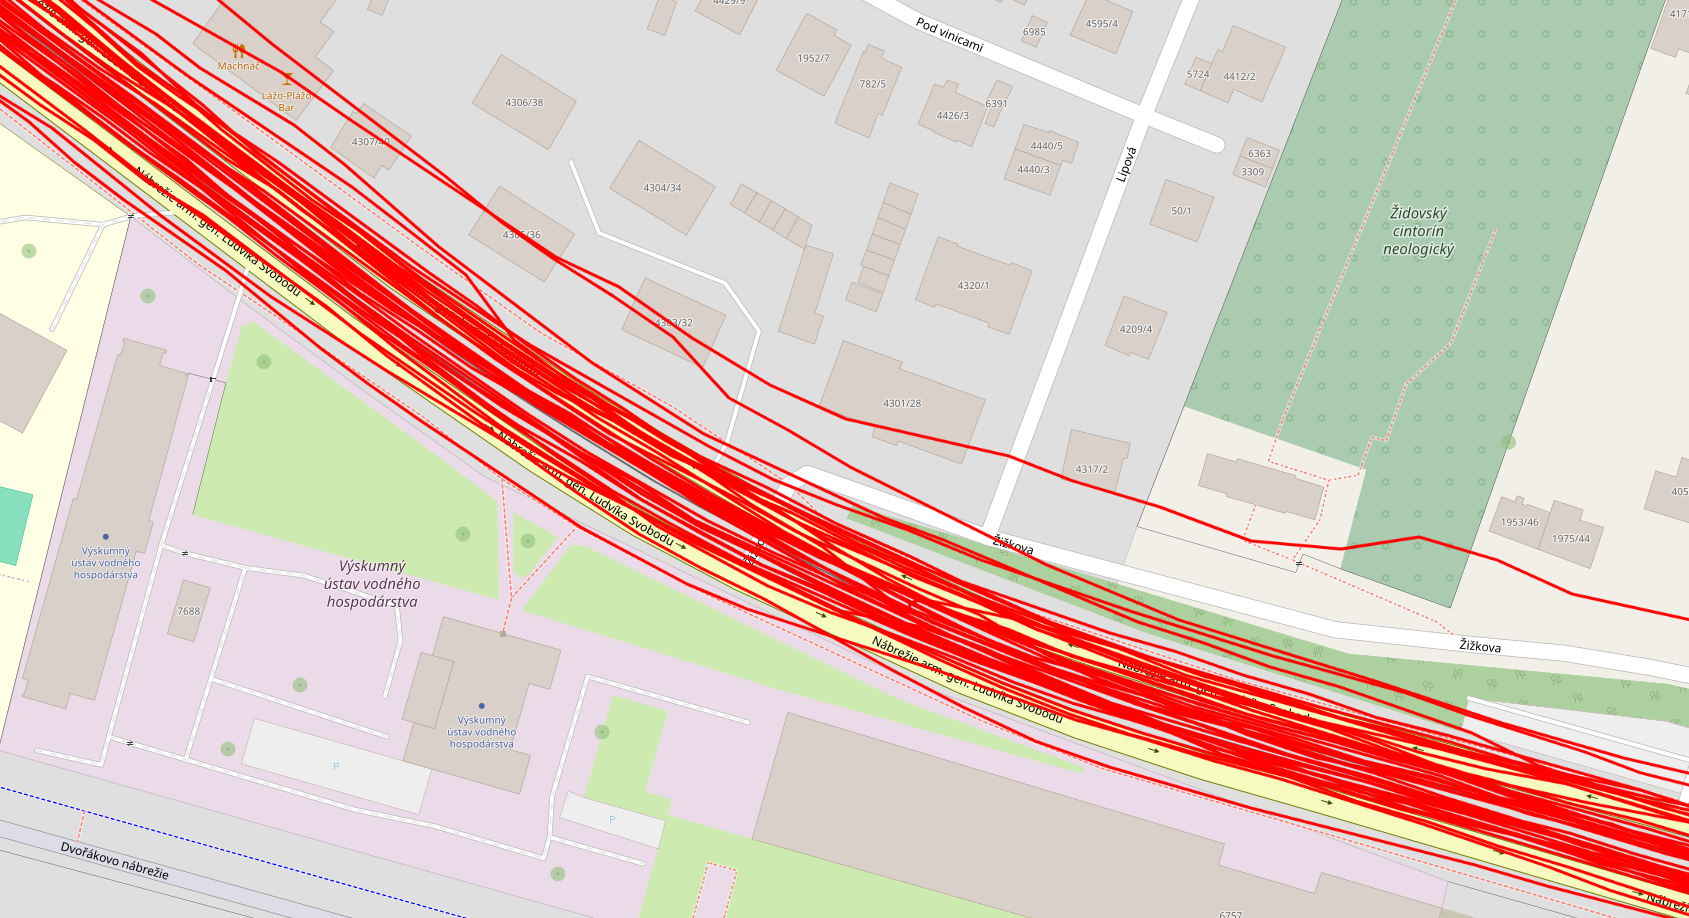
\includegraphics[width=1 \textwidth]{img/problematika_gps/neprehladne_trasy.png}
  \caption{Neprehľadne zobrazené trasy.}
  \label{fig:neprehladne-trasy}
\end{figure}

Pre zlepšenie viditeľnosti a sprehľadnenie mapy všetky trasy upravíme tak, aby sa nachádzali na cestnej sieti, po ktorej sa používateľ reálne pohyboval. Pozrieme sa na rôzne metódy, ktorými túto úpravu dosiahneme. Jednou z nich je \textit{routing}, ktorá nájde trasu medzi každým bodom v pôvodnej trase. Druhou metódou je \textit{map-match}, ktorá vstupné \acrshort{gps} súradnice posunie k cestnej sieti. Tieto dve metódy si bližšie popíšeme v sekcií \ref{section:pripinanie}.

Vďaka týmto úpravám budú všetky trasy ležať na cestnej sieti. Všetky trasy, ktoré sme získali pri pohybe po rovnakej trase budú prekryté a cestná sieť bude viditeľná a mapa prehľadná. Po prejdení myšou po trase sa zobrazí okno, ktoré bude obsahovať názvy prekrytých trás. Taktiež v aplikácii umožníme zobraziť originálne trasy a upravené trasy, pre porovnanie rozdielu. Mapa s upravenými trasami bude vyzerať prehľadne ako na obrázku \ref{fig:prehladne-trasy}. Upravené trasy a pôvodné budú farebne rozlíšené.

\begin{figure}[H]
  \centering
  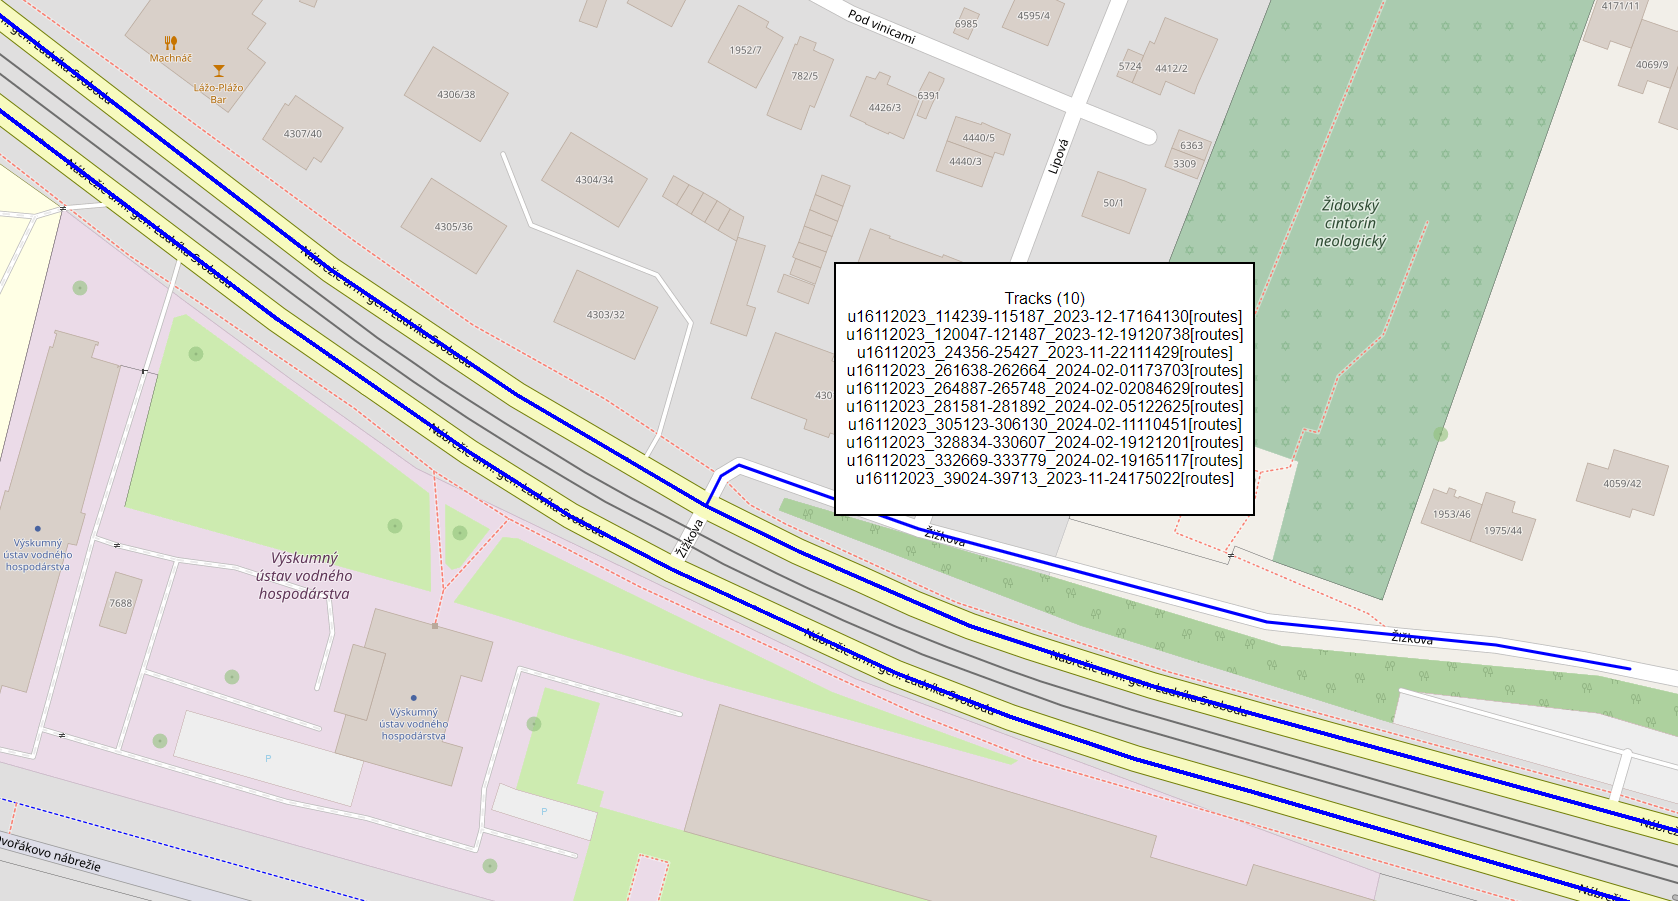
\includegraphics[width=1 \textwidth]{img/problematika_gps/prehladne_trasy.png}
  \caption{Upravené trasy.}
  \label{fig:prehladne-trasy}
\end{figure}

Trasy budú upravené a uložené, aby sa mohli neskôr rýchlejšie vykresliť na mapu. Nebudú sa upravovať pri zobrazovaní, keďže úprava dlhej trasy môže trvať až 200 ms. Zobrazenie celého nahraného ZIP súboru na mape, ktorý môže obsahovať ľubovoľný počet trás spolu s úpravou všetkých trás môže trvať minúty, čo by znepríjemnilo používateľskú skúsenosť.